%---------------
%╔═╗╔═╗╔╦╗╦ ╦╔═╗
%╚═╗║╣  ║ ║ ║╠═╝
%╚═╝╚═╝ ╩ ╚═╝╩  
%---------------
\documentclass[12pt,oneside,a4paper]{report}

% DOCUMENT SETUP
\usepackage[left=3cm, 
			right=2.5cm, 
			top=2.5cm, 
			bottom=2.5cm, 
			includehead, 
			includefoot]{geometry}

% line spacing
\usepackage{setspace}
\setstretch{1,25} % 15/12 --> 1.25

%de­fines Adobe Times Ro­man as de­fault text font
\usepackage{mathptmx}
\usepackage{times} % needed for acronym package

%PDF linking package
\usepackage[hidelinks]{hyperref}

% Language Setup
\usepackage[ngerman]{babel}
% language specific bibliography style
\usepackage[numbers]{natbib}
\usepackage[fixlanguage]{babelbib}
\selectbiblanguage{german}
% bliographystyle setup
% default style names: apalike alphadin ieeetr IEEEtranSN apalike2 alphadin 
% babel specific: babplain, babplai3, babalpha, babunsrt, bababbrv, bababbr3 unsrt 
\bibliographystyle{unsrturl}

% encoding setup
% T1 font encoding for languages that use a latin alphabet
\usepackage[T1]{fontenc} 

% enhanced input encoding handling - utf8 for äÄüÜöÖß...
\usepackage[utf8]{inputenc}
%\usepackage{ucs}%utf8x suppart

% after babel - set chapter string
\AtBeginDocument{\renewcommand{\chaptername}{}}

% enumeration
\usepackage{enumitem}
% tabular extension tabularx
\usepackage{tabularx}

% math packages
\usepackage{amsmath}
\usepackage{nicefrac}
\usepackage{amsthm}
\usepackage{amsbsy}
\usepackage{amssymb}
\usepackage{amsfonts}
\usepackage{MnSymbol}

% patches for latex
\usepackage{fixltx2e}

%special characters
\usepackage{amssymb}
\usepackage{upgreek,textgreek}

% acronym package
\usepackage[printonlyused, footnote]{acronym}

% breakable text in \seqsplit{}
\usepackage{seqsplit}

% \textmu
\usepackage{textcomp}

% package provides a way to compile sections of a document using the same preamble as the main document
\usepackage{subfiles}

% driver-independent color extension - used by listings,tabularx
\usepackage[usenames,dvipsnames,table,xcdraw]{xcolor}

% -- SYNTAX HIGHLIGHTING --
\usepackage{listings}
%% bash command line Syntax Highlighting
\lstdefinestyle{BASH_CMD}{ 
  columns=fullflexible,            % copy pasteable listings
  language=bash,
  basicstyle=\small\sffamily,
  basicstyle   = \small \ttfamily,
  keywordstyle = [1]\small \ttfamily,
  keywordstyle = [2]\small \ttfamily,
  commentstyle = \small \ttfamily,
  numbers=none,
  captionpos=b, 
  breaklines=true,
  numberstyle=\tiny,
  numbersep=3pt,
  frame=tlrb,
  columns=fullflexible,
  backgroundcolor=\color{white!20},
  linewidth=\linewidth,
  literate=                        % replace in code
     {Ö}{{\"O}}1
     {Ä}{{\"A}}1
     {Ü}{{\"U}}1
     {ß}{{\ss}}2
     {ü}{{\"u}}1
     {ä}{{\"a}}1
     {ö}{{\"o}}1
}
 % adds style BASH_CMD
%% Matlab Syntax Highlighting
\colorlet{keyword}{blue!100!black!80}
\colorlet{STD}{Lavender}
\colorlet{comment}{green!90!black!90}
\definecolor{mygreen}{rgb}{0,0.6,0}
\definecolor{mygray}{rgb}{0.5,0.5,0.5}
\definecolor{mymauve}{rgb}{0.58,0,0.82}


\lstdefinestyle{BASH_SCRIPT}{ 
  language     = bash,
  basicstyle   = \footnotesize \ttfamily,
  keywordstyle = [1]\color{keyword}\bfseries,
  keywordstyle = [2]\color{STD}\bfseries,
  commentstyle = \color{mygreen}\itshape,
  backgroundcolor=\color{white},   % choose the background color; you must add \usepackage{color} 
  columns=fullflexible,            % copy pasteable listings
                                   % or \usepackage{xcolor}
  basicstyle=\footnotesize,        % the size of the fonts that are used for the code
  breakatwhitespace=false,         % sets if automatic breaks should only happen at whitespace
  breaklines=true,                 % sets automatic line breaking
  captionpos=b,                    % sets the caption-position to bottom
  extendedchars=true,              % lets you use non-ASCII characters; for 8-bits encodings only,
                                   % does not work with UTF-8
  frame=single,                    % adds a frame around the code
  keepspaces=true,                 % keeps spaces in text, useful for keeping indentation of code
                                   % (possibly needs columns=flexible)
  numbers=left,                    % where to put the line-numbers; possible values are 
                                   % (none, left, right)
  numbersep=5pt,                   % how far the line-numbers are from the code
  numberstyle=\tiny\color{mygray}, % the style that is used for the line-numbers
  rulecolor=\color{black},         % if not set, the frame-color may be changed on line-breaks
                                   % within not-black text (e.g. comments (green here))
  showspaces=false,                % show spaces everywhere adding particular underscores; it
  	                               % overrides 'showstringspaces'
  showstringspaces=false,          % underline spaces within strings only
  showtabs=false,                  % show tabs within strings adding particular underscores
  stepnumber=1,                    % the step between two line-numbers. If it's 1, each line 
                                   % will be numbered
  stringstyle=\color{mymauve},     % string literal style
  tabsize=2,                       % sets default tabsize to 2 spaces
  title=\lstname,                  % set title name
  literate=                        % replace in code
     {Ö}{{\"O}}1
     {Ä}{{\"A}}1
     {Ü}{{\"U}}1
     {ß}{{\ss}}2
     {ü}{{\"u}}1
     {ä}{{\"a}}1
     {ö}{{\"o}}1
} % adds style BASH_SCRIPT
% Matlab Syntax Highlighting
\colorlet{keyword}{blue!100!black!80}
\colorlet{STD}{red}
\colorlet{comment}{green!90!black!90}
\definecolor{mygreen}{rgb}{0,0.6,0}
\definecolor{mygray}{rgb}{0.5,0.5,0.5}
\definecolor{mymauve}{rgb}{0.58,0,0.82}


\lstdefinestyle{LATEX}{ 
  language     = [LaTeX]{TeX},
  basicstyle   = \footnotesize \ttfamily,
  keywordstyle = [1]\color{keyword}\bfseries,
  keywordstyle = [2]\color{comment}\bfseries,
  commentstyle = \color{mygray}\itshape,
  %backgroundcolor=\color{white},   % choose the background color; you must add \usepackage{color} 
                                   % or \usepackage{xcolor}
  basicstyle=\footnotesize,        		   % the size of the fonts that are used for the code
  breakatwhitespace=false,         % sets if automatic breaks should only happen at whitespace
  columns=fullflexible,            % copy pasteable listings
  breaklines=true,                 % sets automatic line breaking
  captionpos=c,                    % sets the caption-position to bottom
  extendedchars=true,              % lets you use non-ASCII characters; for 8-bits encodings only,
                                   % does not work with UTF-8
  frame=single,                    % adds a frame around the code
  keepspaces=true,                 % keeps spaces in text, useful for keeping indentation of code
                                   % (possibly needs columns=flexible)
  numbers=left,                    % where to put the line-numbers; possible values are 
                                   % (none, left, right)
  numbersep=4pt,                   % how far the line-numbers are from the code
  numberstyle=\tiny\color{mygray}, % the style that is used for the line-numbers
  rulecolor=\color{black},         % if not set, the frame-color may be changed on line-breaks
                                   % within not-black text (e.g. comments (green here))
  showspaces=false,                % show spaces everywhere adding particular underscores; it
  	                               % overrides 'showstringspaces'
  showstringspaces=false,          % underline spaces within strings only
  showtabs=false,                  % show tabs within strings adding particular underscores
  stepnumber=1,                    % the step between two line-numbers. If it's 1, each line 
                                   % will be numbered
  stringstyle=\color{mymauve},     % string literal style
  tabsize=2,                       % sets default tabsize to 2 spaces
  title=\lstname,                  % set title name
  literate=                        % replace in code
     {Ö}{{\"O}}1
     {Ä}{{\"A}}1
     {Ü}{{\"U}}1
     {ß}{{\ss}}2
     {ü}{{\"u}}1
     {ä}{{\"a}}1
     {ö}{{\"o}}1
} % adds style LATEX
%% Matlab Syntax Highlighting
\colorlet{keyword}{blue!100!black!80}
\colorlet{STD}{Lavender}
\colorlet{comment}{green!90!black!90}
\definecolor{mygreen}{rgb}{0,0.6,0}
\definecolor{mygray}{rgb}{0.5,0.5,0.5}
\definecolor{mymauve}{rgb}{0.58,0,0.82}


\lstdefinestyle{MATLAB}{ 
  language     = Matlab,
  basicstyle   = \footnotesize \ttfamily,
  keywordstyle = [1]\color{keyword}\bfseries,
  keywordstyle = [2]\color{STD}\bfseries,
  commentstyle = \color{mygreen}\itshape,
  backgroundcolor=\color{white},   % choose the background color; you must add \usepackage{color} 
                                   % or \usepackage{xcolor}
  basicstyle=\footnotesize,        % the size of the fonts that are used for the code
  breakatwhitespace=false,         % sets if automatic breaks should only happen at whitespace
  columns=fullflexible,            % copy pasteable listings
  breaklines=false,                % sets automatic line breaking
  captionpos=c,                    % sets the caption-position to bottom
  extendedchars=true,              % lets you use non-ASCII characters; for 8-bits encodings only,
                                   % does not work with UTF-8
  frame=single,                    % adds a frame around the code
  keepspaces=true,                 % keeps spaces in text, useful for keeping indentation of code
                                   % (possibly needs columns=flexible)
  numbers=left,                    % where to put the line-numbers; possible values are 
                                   % (none, left, right)
  numbersep=5pt,                   % how far the line-numbers are from the code
  numberstyle=\tiny\color{mygray}, % the style that is used for the line-numbers
  rulecolor=\color{black},         % if not set, the frame-color may be changed on line-breaks
                                   % within not-black text (e.g. comments (green here))
  showspaces=false,                % show spaces everywhere adding particular underscores; it
  	                               % overrides 'showstringspaces'
  showstringspaces=false,          % underline spaces within strings only
  showtabs=false,                  % show tabs within strings adding particular underscores
  stepnumber=1,                    % the step between two line-numbers. If it's 1, each line 
                                   % will be numbered
  stringstyle=\color{mymauve},     % string literal style
  tabsize=2,                       % sets default tabsize to 2 spaces
  title=\lstname,                  % set title name
  literate=                        % replace in code
     {Ö}{{\"O}}1
     {Ä}{{\"A}}1
     {Ü}{{\"U}}1
     {ß}{{\ss}}2
     {ü}{{\"u}}1
     {ä}{{\"a}}1
     {ö}{{\"o}}1
} % adds style MATLAB
% Matlab Syntax Highlighting
\colorlet{keyword}{blue!100!black!80}
\colorlet{STD}{Lavender}
\colorlet{comment}{green!90!black!90}
\definecolor{mygreen}{rgb}{0,0.6,0}
\definecolor{mygray}{rgb}{0.5,0.5,0.5}
\definecolor{mymauve}{rgb}{0.58,0,0.82}


\lstdefinestyle{PYTHON}{ 
  language     = Python,
  basicstyle   = \footnotesize \ttfamily,
  keywordstyle = [1]\color{keyword}\bfseries,
  keywordstyle = [2]\color{STD}\bfseries,
  commentstyle = \color{mygreen}\itshape,
  backgroundcolor=\color{white},   % choose the background color; you must add \usepackage{color} 
                                   % or \usepackage{xcolor}
  basicstyle=\footnotesize,        % the size of the fonts that are used for the code
  columns=fullflexible,            % copy pasteable listings
  breakatwhitespace=false,         % sets if automatic breaks should only happen at whitespace
  breaklines=false,                % sets automatic line breaking
  captionpos=c,                    % sets the caption-position to bottom
  extendedchars=true,              % lets you use non-ASCII characters; for 8-bits encodings only,
                                   % does not work with UTF-8
  frame=single,                    % adds a frame around the code
  keepspaces=true,                 % keeps spaces in text, useful for keeping indentation of code
                                   % (possibly needs columns=flexible)
  numbers=left,                    % where to put the line-numbers; possible values are 
                                   % (none, left, right)
  numbersep=5pt,                   % how far the line-numbers are from the code
  numberstyle=\tiny\color{mygray}, % the style that is used for the line-numbers
  rulecolor=\color{black},         % if not set, the frame-color may be changed on line-breaks
                                   % within not-black text (e.g. comments (green here))
  showspaces=false,                % show spaces everywhere adding particular underscores; it
  	                               % overrides 'showstringspaces'
  showstringspaces=false,          % underline spaces within strings only
  showtabs=false,                  % show tabs within strings adding particular underscores
  stepnumber=1,                    % the step between two line-numbers. If it's 1, each line 
                                   % will be numbered
  stringstyle=\color{mymauve},     % string literal style
  tabsize=2,                       % sets default tabsize to 2 spaces
  title=\lstname,                  % set title name
  literate=                        % replace in code
     {Ö}{{\"O}}1
     {Ä}{{\"A}}1
     {Ü}{{\"U}}1
     {ß}{{\ss}}2
     {ü}{{\"u}}1
     {ä}{{\"a}}1
     {ö}{{\"o}}1
} % adds style PYTHON
%% Matlab Syntax Highlighting
\colorlet{keyword}{blue!100!black!80}
\colorlet{STD}{Lavender}
\colorlet{comment}{green!90!black!90}
\definecolor{mygreen}{rgb}{0,0.6,0}
\definecolor{mygray}{rgb}{0.5,0.5,0.5}
\definecolor{mymauve}{rgb}{0.58,0,0.82}


\lstdefinestyle{CPP}{ 
  language     = C++,
  basicstyle   = \footnotesize \ttfamily,
  keywordstyle = [1]\color{keyword}\bfseries,
  keywordstyle = [2]\color{STD}\bfseries,
  commentstyle = \color{mygreen}\itshape,
  backgroundcolor=\color{white},   % choose the background color; you must add \usepackage{color} 
                                   % or \usepackage{xcolor}
  columns=fullflexible,            % copy pasteable listings
  basicstyle=\footnotesize,        % the size of the fonts that are used for the code
  breakatwhitespace=false,         % sets if automatic breaks should only happen at whitespace
  breaklines=false,                % sets automatic line breaking
  captionpos=c,                    % sets the caption-position to bottom
  extendedchars=true,              % lets you use non-ASCII characters; for 8-bits encodings only,
                                   % does not work with UTF-8
  frame=single,                    % adds a frame around the code
  keepspaces=true,                 % keeps spaces in text, useful for keeping indentation of code
                                   % (possibly needs columns=flexible)
  numbers=left,                    % where to put the line-numbers; possible values are 
                                   % (none, left, right)
  numbersep=5pt,                   % how far the line-numbers are from the code
  numberstyle=\tiny\color{mygray}, % the style that is used for the line-numbers
  rulecolor=\color{black},         % if not set, the frame-color may be changed on line-breaks
                                   % within not-black text (e.g. comments (green here))
  showspaces=false,                % show spaces everywhere adding particular underscores; it
  	                               % overrides 'showstringspaces'
  showstringspaces=false,          % underline spaces within strings only
  showtabs=false,                  % show tabs within strings adding particular underscores
  stepnumber=1,                    % the step between two line-numbers. If it's 1, each line 
                                   % will be numbered
  stringstyle=\color{mymauve},     % string literal style
  tabsize=2,                       % sets default tabsize to 2 spaces
  title=\lstname,                  % set title name
  literate=                        % replace in code
     {Ö}{{\"O}}1
     {Ä}{{\"A}}1
     {Ü}{{\"U}}1
     {ß}{{\ss}}2
     {ü}{{\"u}}1
     {ä}{{\"a}}1
     {ö}{{\"o}}1
} % adds style CPP
%% Matlab Syntax Highlighting
\colorlet{keyword}{blue!100!black!80}
\colorlet{STD}{Lavender}
\colorlet{comment}{green!90!black!90}
\definecolor{mygreen}{rgb}{0,0.6,0}
\definecolor{mygray}{rgb}{0.5,0.5,0.5}
\definecolor{mymauve}{rgb}{0.58,0,0.82}


\lstdefinestyle{C}{ 
  language     = C,
  basicstyle   = \footnotesize \ttfamily,
  keywordstyle = [1]\color{keyword}\bfseries,
  keywordstyle = [2]\color{STD}\bfseries,
  commentstyle = \color{mygreen}\itshape,
  backgroundcolor=\color{white},   % choose the background color; you must add \usepackage{color} 
  columns=fullflexible,            % copy pasteable listings
                                   % or \usepackage{xcolor}
  basicstyle=\footnotesize,        % the size of the fonts that are used for the code
  breakatwhitespace=false,         % sets if automatic breaks should only happen at whitespace
  breaklines=false,                % sets automatic line breaking
  captionpos=c,                    % sets the caption-position to bottom
  extendedchars=true,              % lets you use non-ASCII characters; for 8-bits encodings only,
                                   % does not work with UTF-8
  frame=single,                    % adds a frame around the code
  keepspaces=true,                 % keeps spaces in text, useful for keeping indentation of code
                                   % (possibly needs columns=flexible)
  numbers=left,                    % where to put the line-numbers; possible values are 
                                   % (none, left, right)
  numbersep=5pt,                   % how far the line-numbers are from the code
  numberstyle=\tiny\color{mygray}, % the style that is used for the line-numbers
  rulecolor=\color{black},         % if not set, the frame-color may be changed on line-breaks
                                   % within not-black text (e.g. comments (green here))
  showspaces=false,                % show spaces everywhere adding particular underscores; it
  	                               % overrides 'showstringspaces'
  showstringspaces=false,          % underline spaces within strings only
  showtabs=false,                  % show tabs within strings adding particular underscores
  stepnumber=1,                    % the step between two line-numbers. If it's 1, each line 
                                   % will be numbered
  stringstyle=\color{mymauve},     % string literal style
  tabsize=2,                       % sets default tabsize to 2 spaces
  title=\lstname,                  % set title name
  literate=                        % replace in code
     {Ö}{{\"O}}1
     {Ä}{{\"A}}1
     {Ü}{{\"U}}1
     {ß}{{\ss}}2
     {ü}{{\"u}}1
     {ä}{{\"a}}1
     {ö}{{\"o}}1
} % adds style C
%% JSON Syntax Highlighting
\colorlet{keyword}{blue!100!black!80}
\colorlet{STD}{Lavender}
\colorlet{comment}{green!90!black!90}
\definecolor{mygreen}{rgb}{0,0.6,0}
\definecolor{mygray}{rgb}{0.5,0.5,0.5}
\definecolor{mymauve}{rgb}{0.58,0,0.82}

\newcommand\JSONnumbervaluestyle{\color{blue}}
\newcommand\JSONstringvaluestyle{\color{red}}

\newif\ifcolonfoundonthisline

\makeatletter

\lstdefinelanguage{json}
{
  showstringspaces    = false,
  keywords            = {false,true},
  alsoletter          = 0123456789.,
  morestring          = [s]{"}{"},
  morestring          = [s]{'}{'},
  stringstyle         = \ifcolonfoundonthisline\JSONstringvaluestyle\fi,
  MoreSelectCharTable =%
    \lst@DefSaveDef{`:}\colon@json{\processColon@json},
  basicstyle          = \ttfamily,
  keywordstyle        = \ttfamily\bfseries,
}

% flip the switch if a colon is found in Pmode
\newcommand\processColon@json{
  \colon@json%
  \ifnum\lst@mode=\lst@Pmode%
    \global\colonfoundonthislinetrue%
  \fi
}

\lst@AddToHook{Output}{%
  \ifcolonfoundonthisline%
    \ifnum\lst@mode=\lst@Pmode%
      \def\lst@thestyle{\JSONnumbervaluestyle}%
    \fi
  \fi
  %override by keyword style if a keyword is detected!
  \lsthk@DetectKeywords% 
}

% reset the switch at the end of line
\lst@AddToHook{EOL}%
  {\global\colonfoundonthislinefalse}

\makeatother



\lstdefinestyle{JSON}{ 
  language     = json,
  basicstyle   = \footnotesize \ttfamily,
  keywordstyle = [1]\color{keyword}\bfseries,
  keywordstyle = [2]\color{STD}\bfseries,
  commentstyle = \color{mygreen}\itshape,
  backgroundcolor=\color{white},   % choose the background color; you must add \usepackage{color} 
                                   % or \usepackage{xcolor}
  basicstyle=\footnotesize,        % the size of the fonts that are used for the code
  columns=fullflexible,            % copy pasteable listings
  breakatwhitespace=false,         % sets if automatic breaks should only happen at whitespace
  breaklines=false,                % sets automatic line breaking
  captionpos=c,                    % sets the caption-position to bottom
  extendedchars=true,              % lets you use non-ASCII characters; for 8-bits encodings only,
                                   % does not work with UTF-8
  frame=single,                    % adds a frame around the code
  keepspaces=true,                 % keeps spaces in text, useful for keeping indentation of code
                                   % (possibly needs columns=flexible)
  numbers=left,                    % where to put the line-numbers; possible values are 
                                   % (none, left, right)
  numbersep=5pt,                   % how far the line-numbers are from the code
  numberstyle=\tiny\color{mygray}, % the style that is used for the line-numbers
  rulecolor=\color{black},         % if not set, the frame-color may be changed on line-breaks
                                   % within not-black text (e.g. comments (green here))
  showspaces=false,                % show spaces everywhere adding particular underscores; it
  	                               % overrides 'showstringspaces'
  showstringspaces=false,          % underline spaces within strings only
  showtabs=false,                  % show tabs within strings adding particular underscores
  stepnumber=1,                    % the step between two line-numbers. If it's 1, each line 
                                   % will be numbered
  stringstyle=\color{mymauve},     % string literal style
  tabsize=2,                       % sets default tabsize to 2 spaces
  title=\lstname,                  % set title name
  literate=                        % replace in code
     {Ö}{{\"O}}1
     {Ä}{{\"A}}1
     {Ü}{{\"U}}1
     {ß}{{\ss}}2
     {ü}{{\"u}}1
     {ä}{{\"a}}1
     {ö}{{\"o}}1
} % adds style JSON

% HEADLINE CFG
\usepackage{fancyhdr} % Headers and footers
\usepackage{lastpage}
\usepackage{nopageno}
\setlength{\headheight}{1.5cm}
\pagestyle{fancy} % All pages have headers and footers
\fancyhead{} % Blank out the default header
\fancyfoot{} % Blank out the default footer
\fancyhead[L]{}
\fancyhead[C]{}
\fancyhead[R]{}
\fancyfoot[L]{}
\fancyfoot[C]{\thepage}
\fancyfoot[R]{}
% override plain page style for \part, \chapter or 
% \maketitle, which implicit specifies plain page style
\fancypagestyle{plain} 
{
	\fancyhead[L]{}
	\fancyhead[C]{}
	\fancyhead[R]{}
	\fancyfoot[L]{}
	\fancyfoot[C]{\thepage}
	\fancyfoot[R]{}
}
% set list pagestyle
\fancypagestyle{lists} 
{
	\fancyhead[L]{}
	\fancyhead[C]{}
	\fancyhead[R]{}
	\fancyfoot[L]{}
	\fancyfoot[C]{\thepage}
	\fancyfoot[R]{}
}

\renewcommand{\chaptermark}[1]{\markright{#1}{}}
\renewcommand{\sectionmark}[1]{\markright{#1}{}}
\renewcommand{\headrulewidth}{0pt}
\renewcommand{\footrulewidth}{0pt}

	
\usepackage{verbatim}
\usepackage{graphicx}
\usepackage{epstopdf}

% floating prevention packages
\usepackage{float}    % used with [H] positioning parameter
\usepackage{placeins} % \FloatBarrier 

% tikz packages
\usepackage{tikz}
\usepackage{caption}
\usepackage[list=true,listformat=simple]{subcaption}
\usepackage{standalone}
\usepackage{pgfplots}
\usepackage{graphicx}
\graphicspath{{media/}}

% include only specified tex files - uncommend unneeded
\includeonly{preface/cover,
             preface/abstract,
             preface/tableofcontents,
             preface/listoffigures,
             preface/listoftables,
             preface/listofabbreviations,
             appendix/bibliography}

% hyperref customization
\hypersetup{
	pdftitle    ={IoT Sensor}, % title
	pdfsubject	={IoT Sensor}, % subject of the document
	pdfauthor	={Fabian Gendusa \& Thomas Gnädig}, % author
	pdfkeywords	={}, % list of keywords
	pdfcreator	={}, % creator of the document
	pdfproducer	={}, % producer of the document
	colorlinks=false, % false: boxed links; true: colored links
	linkcolor=red, % color of internal links (change box color with linkbordercolor)
    citecolor=green, % color of links to bibliography
    filecolor=magenta, % color of file links
    urlcolor=cyan, % color of external links
	%bookmarks=true, % show bookmarks bar?
	unicode=true, % non-Latin characters in Acrobat’s bookmarks
	pdftoolbar=true, % show Acrobat’s toolbar?
	pdfmenubar=true, % show Acrobat’s menu?
    pdffitwindow=false, % window fit to page when opened
	pdfnewwindow=true % links in new PDF window
}

%-----------------------------------------
% ╔╗ ╔═╗╔═╗╦╔╗╔  ╔╦╗╔═╗╔═╗╦ ╦╔╦╗╔═╗╔╗╔╔╦╗ 
% ╠╩╗║╣ ║ ╦║║║║   ║║║ ║║  ║ ║║║║║╣ ║║║ ║  
% ╚═╝╚═╝╚═╝╩╝╚╝  ═╩╝╚═╝╚═╝╚═╝╩ ╩╚═╝╝╚╝ ╩  
%-----------------------------------------

\begin{document}
\pagenumbering{Roman} 

%\setcounter{section}{0}

\begin{titlepage}

\vspace*{-3.5cm}

\begin{flushleft}
\hspace*{-1cm} 

\begin{figure}
\begin{subfigure}[c]{0.7\textwidth}

\includegraphics[width=\textwidth]{preface/htwg-logo}
\end{subfigure}

\end{figure}
\end{flushleft}

\vspace{5cm}

\begin{center}
	\large{
		\textbf{Teamprojekt Modulare Plattform für intelligente IoT-Sensoren} \\[.2cm]
	}
	\small{
		\textbf{Konstanz den, \today}	}\\[1cm]
		
	
\vspace{6cm}
	
	
	\large{
		\begin{flushleft}
			\begin{tabular}{ll}
				\textbf{Team:} & Fabian Gendusa \& Thomas Gnädig \\
				\textbf{Zeitraum:} & WS 16/17 \\
				Fachbetreuer: & I. Schoppa \\
				Fakultät: & Informatik \\
				Studiengang: & Angewandte Informatik \\
			\end{tabular}
		\end{flushleft}
	}
	

\end{center}

\end{titlepage}
\thispagestyle{empty}




%--------------------------
% ╔═╗╦ ╦╔═╗╔═╗╔╦╗╔═╗╦═╗╔═╗ 
% ║  ╠═╣╠═╣╠═╝ ║ ║╣ ╠╦╝╚═╗ 
% ╚═╝╩ ╩╩ ╩╩   ╩ ╚═╝╩╚═╚═╝ 
%--------------------------

\pagenumbering{arabic} 
\setcounter{page}{1}

%
% CHAPTER Vorwort
%
%
% CHAPTER Vorwort
%
\chapter{Vorwort}
\label{chap:Vorwort}

%Motivation zum Projekt
Unnötig?







%
\chapter{Das Projekt}
\label{chap:beschreibung}

\section{Projekt Beschreibung}
Im Rahmen des Studiums ist ein mit 12 ECTS gewichtetes Teamprojekt vorgesehen.
Das Projekt IoT Sensor kombiniert drei selbst erstellte Platinen zu einem funktionierenden System.

Auf der Hauptplatine wird ein Mikrocontroller der Art MSP470FR und drei PMOD Schnittstellen angebracht. Über die PMOD Stecker soll mit den anderen Board kommuniziert werden.

Die Kommunikationsplatine wird mit USB am PC verbunden und mithilfe des FT231X auf UART umgewandelt. Das umgewandelte Signal wird dann über einen PMOD Stecker via UART an das Main-Board weitergeleitet. auf der Platine befindet sich auch eine galvanische Trennung, welche den Stromkreis des Computers vom Stromkreis des Mikrocontrollers trennt. Hierfür ist der ADUM1401 verantwortlich, welcher das Signal über Lichtwellen weiter gibt.

Die Anzeige Platine stellt eine 7 Segmentanzeige zur Verfügung, welche die Visualisierung von Beispielsweise Sensorwerten übernimmt. hierzu Dient der AS1108 welcher die Übersetzung einer Zahl auf die Sieben Segmentanzeige übernimmt. Die Zahlen werden über SPI vom Mainboard erhalten.

Die Sensorplatine, nicht teil des Projekts, wird auch über SPI angesprochen und liefert Messwerte an das Main-Board. Kann bei bedarf  bereits Fertig gekauft werden.

\section{Arbeitsschritte}

\subsection{Bauteilsuche}
Nachdem die Vorgabe vollständig ist, kann mit der Bauteilsuche begonnen werden. Einige Teile waren auch bereits vorgegeben. Kriterien beim auswählen der Bauteile waren:

\begin{itemize}
	\item die Funktion, Angaben müssen erfüllt werden
	\item die Verfügbarkeit, Teile müssen einzeln bestellbar und auch in Zukunft noch Angeboten sein
	\item der Preis
\end{itemize}

\subsection{Platinen Design}
Nachdem alle Teile gefunden sind und auch alle Datenblätter vorliegen, kann mit dem Design der Platine begonnen werden.
hierzu haben wir das Tool Pulsonix verwendet, nachdem der Schaltplan hierin entworfen war, konnte das Schematic erstellt werden, die größte Hürde hierbei war das einstellen des korrekten Rasters für Bauteile und Vias.
zu beachten war, dass manche Bauteile möglichst nah an anderen Bauteilen angebracht werden, so zb beim FT231X, wo ein differentielles Signal anlag.
Auch zu beachten war an den PMOD Steckern sollten zwei Kondensatoren angebracht werden um Störsignale welche beispielsweise beim anstecken entstehen raus zu filtern.

\subsection{Hardware bestücken}
Die Hardware wurde bei \url{www.digikey.com} bestellt und war innerhalb kurzer zeit angeliefert. Um die Platinen zu bestellen, mussten zunächst Gerberfiles erstellt werden, welche dann an Q-print electronic GmbH geschickt wurde.
Zum bestücken der Platine war Teamarbeit gefragt, während einer das Bauteil möglichst exakt auf den kleinen Pads positioniert muss der Zweite das erste Beinchen fest löten. die wohl größte Herausforderung hierbei war das befestigen des FT321X auf der Kommunikationsplatine. Nachdem diese Herausforderung gemeistert war, stellten die anderen Bauteile keine größeren Probleme mehr dar.
Als Änderung für neue Platinen wäre bei der Anzeigenplatine ein Größerer $RSET$ Widerstand einzubauen, da der eingebaute 10 $k\Omega$ etwas zu klein dimensioniert ist. wenigstens 11,35 $k\Omega$ siehe Datenblatt AS1108 Seite 9.

\subsection{Softwareentwicklung}
Es musste nicht nur ein Treiber für den MSP geschrieben werden um über UART und SPI mit unseren Boards zu kommunizieren, sondern auch ein Treiber, welcher die Kommunikation zwischen PC und Kommunikationsplatine übernimmt. Die genauere beschreibung folgt im nächsten Kapitel.



%
\chapter{Entwickelte-Software}
\label{chap:Anwendung}

\section{Python}
Für die Programmierung, um auf das Kommunikationsboard zugreifen zu können, haben wir uns für Python entschieden, da es hier relativ einfache und schnelle wege gibt um c librarys einzubinden und zu benutzen.  Wir greifen hier auf die vom Hersteller bereitgestellte library "ftd2xx" zurück.

\subsection{MSP430connect.py}
Dieses Script dient zur Übertragung eines durch CCS erstellten Programms mithilfe des USB-UART-Konverters auf den Microcontroller. Es kann mit dem Parameter -p [Dateipfad] ausgeführt werden, wobei dann das Programm heruntergeladen wird. Wird es ohne Angabe von Parametern gestartet öffnet sich ein textuelles Benutzerinterface. Mit dem Parameter h kann eine kleine Hilfe zum Programm angezeigt werden. Wie die Das Programm zum herunterladen auf den Microkontroller mit CCS erstellt werden muss, wird auch in dieser beschrieben.
Das Script verwendet unseren MSP430.py Treiber, welcher einfache Methoden zum öffnen eines Devices, lesen und schreiben sowie zurücksetzen dieses Devices anbietet. Diese Methoden können für weitere Programme genutzt werden.


\subsection{Übersicht Dateien}

\begin{tabular}{|l|p{11cm}| }
\hline
Dateiname & Beschreibung \\ \hline
FT\_declarations.py & Enthält Deklarationen für den Wrapper des FT2XX \\ \hline
FT\_Device.py & Wrapper-Klasse für die Kommunikation mit dem FT2XX. \\ \hline
MSP430.py	& Klasse, zur Kommunikation mit dem Bootstraploader. Bietet Funktionen zum Schreiben, Lesen der seriellen Schnittstelle. Weiter auch die Funktion, um ein Programm auf den Microkontroller zu laden. \\ \hline
ProgrammContainer.py  & Hilfsklasse zum Parsen und Speichern des Programms, das auf den Mikrokontroller zu laden ist. \\ \hline
\end{tabular} 


\section{C-Code}

\subsection{Einstiegs Codes}
Da wir uns das erste mal mit CCS und dem MSP430FR befassen, haben wir uns zunächst ein paar simple Anwendungen überlegt um ein Gefühl für die Umgebung zu bekommen. Hierzu haben wir vor allem die auf dem Experimentierboard angebrachten LEDs als Ausgabe verwendet um möglichst schnell und einfach ein Feedback zu erhalten. Eine einfache Anwendung war das erstellen eines Lauflichts, welches über Tastendruck zusätzlich beeinflusst werden konnte \tiny(CD\textbackslash Code\textbackslash runled.c)\normalsize. Auch den auf dem Board eingebauten Wärmesensor haben wir ausgelesen und dessen wert direkt an die LEDs angelegt \tiny(CD\textbackslash Code\textbackslash adc.c)\normalsize. Dass sich die Zahl beim auflegen des Fingers auf den Sensor verändert hat war ein kleines aber feines Erfolgserlebnis.

\subsection{UART}
Für die Kommunikation von UART haben wir einen kleinen Treiber geschrieben, welcher zum initialisieren von maximal 2 UART Schnittstellen verwendet werden kann, eine Funktion um eine Zeichenkette zu lesen oder schreiben wird auch bereit gestellt \tiny(CD\textbackslash Code\textbackslash UART\textbackslash uart.c|h)\normalsize.

\subsection{SPI}
Auch für die beiden SPI Schnittstellen wurde ein Treiber geschrieben, dieser ist ebenfalls auf der CD vorhanden\tiny(CD\textbackslash Code\textbackslash SPI\textbackslash spi.c|h)\normalsize.
Ein Beispielcode zum ansprechen der Siebensegmentanzeige befindet sich ebenfalls in diesem Ordner, hier ist es uns bis heute leider nicht gelungen, den Treiberbaustein korrekt zu konfigurieren, die Funktionalität der SPI Schnittstelle ist aber bereits geprüft und funktioniert wie in diesem Beispielcode beschrieben.


%
\chapter{Hilfsmittel/Arbeitsumgebung}
\label{chap:arbeit}

Zum Erstellen des Schaltplans und der Gerberfiles haben wir das auf den Laborrechnern bereitgestellte Tool Pulsonix verwendet.\\
Die Python Programmierung haben wir im Notepad++ durchgeführt.\\
Um den MSP430FR zu beschreiben griffen wir auf das vom Hersteller bereitgestellte Tool CCS zurück.

\subsection{Installation und anwendung des CCS}
\raggedright
Die aktuellste Version des CCS kann unter folgender URL bei ti direkt heruntergeladen werden \url{http://processors.wiki.ti.com/index.php/Download_CCS}.
Nach dem Ausführen der css\_setup.exe sollte im Schritt "processor support" wenigstens die Familie MSP430 wie in folgendem Screenshot gezeigt ausgewählt werden.\\
	\centering
	\fbox{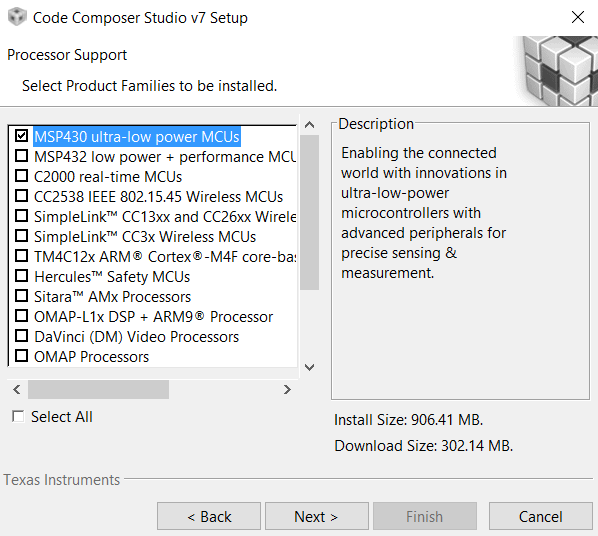
\includegraphics[width=0.5\textwidth]{media/ccs.PNG}}\\
\raggedright	
Nach der Installation des Programms kann ein Workspace angelegt oder ein bereits bestehender genutzt werden.
Beim Erstellen eines neuen Projektes sollte darauf geachtet werden, dass auch der richtige Microcontroller ausgewählt ist. Folgender Screenshot zeigt die korrekte Einstellung\\
	\centering
	\fbox{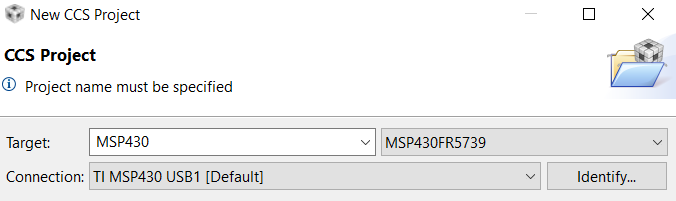
\includegraphics[width=0.5\textwidth]{media/ccs2.PNG}}\\
\raggedright	
Durch diese Auswahl werden bereits die richtigen Bibliotheken eingebunden.
Hier kann auch ein kleines Beispielprogramm erstellt werden, welches eine LED blinken lässt.
Die weitere Programmierung ist wie in herkömmlichen Entwicklungsumgebungen.
Eine nette und hilfreiche Erweiterung ist der Debugmodus, welcher uns schon oft weiter geholfen hat. Hier kann das Programm auf dem MSP430 direkt laufengelassen, angehalten und fortgesetzt werden.


Ein bereits fertiger Workspace-Ordner mit allen hier aufgelisteten Programme ist auch auf der CD zu finden.


\subsection{Erstellen des Download-Files}
Ein Programm, das mit dem MSP430Connect Skript auf den Mikrokontroller geladen werden soll muss in einem bestimmten Dateiformat vorliegen. Zur Erstellung dieser Datei müssen im Code Composer Studio (CCS) zuerst einige Einstellungen vorgenommen werden.

1. unter 'Build' Configuration auf Release stellen

2. unter 'MSP430 Hex Utility' haken bei Enable MSP430 Hex Utility aktivieren

3. unter 'Output Format Options' das Output format auf Output TI\_TXT hex Format setzen

4. Build Release ausführen, 'projektname'.txt liegt jetzt im workspace

Diese 'projektname'.txt muss dann dem MSP430Connect Skript als Parameter übergeben werden.


\end{document}
%------------------------------------
% ╔═╗╔╗╔╔╦╗  ╔╦╗╔═╗╔═╗╦ ╦╔╦╗╔═╗╔╗╔╔╦╗
% ║╣ ║║║ ║║   ║║║ ║║  ║ ║║║║║╣ ║║║ ║ 
% ╚═╝╝╚╝═╩╝  ═╩╝╚═╝╚═╝╚═╝╩ ╩╚═╝╝╚╝ ╩ 
%------------------------------------